\documentclass[10pt]{article}
\usepackage[margin=0.78in]{geometry}
\usepackage{graphicx,booktabs,longtable,amsmath,hyperref,xcolor}
\hypersetup{colorlinks=true,urlcolor=blue}
\setlength{\parindent}{0pt}\setlength{\parskip}{6pt}
\begin{document}
\title{Aero Challenge 01\\A Reference-Withheld NACA 0012 Prediction Experiment}
\author{Alex Blythe / Aero engineering record}\date{September 2026}\maketitle
\begin{abstract}
A nominal two-dimensional steady-RANS prediction was preregistered, executed on three grids at each of 18 angles, and frozen before the experimental reference was revealed. The numerical disposition is FAIL; experimental coefficient comparison is FAIL; overall status is FAIL. This result is preserved without post-reveal tuning.
\end{abstract}
\section{Decision and scope}
Complete nominal steady-RANS prediction retained. Numerical acceptance failed; no design-ready or validated prediction is claimed, irrespective of later coefficient agreement. Setup supervisor was source-exposed; solver execution was reference-withheld. No physical-time average, exact grit equivalence, or universal validation is claimed.
\section{What was actually tested}
NASA TM-4074 Table XIII, first subtable: NACA0012, Mach0.15, Reynolds number5.95 million, fixed transition strips at5 percent chord. The complete18-point CL/CD polar is retained. This is not a Cp-field comparison, an as-built reconstruction or a certified design calculation.
\section{Independence limitation}
The solver containers had no reference or decryption key. However, the source-exposed supervisor authored the numerical setup. This is runtime reference withholding, not double-blind source selection or independently blinded supervisory design. A fresh input-only model review does not remove that limitation.
\section{Top-level results}
0 of 54 cases passed their applicable individual numerical gates; 2 of 18 medium/fine comparisons passed. 54 meshes retained failed checkMesh checks under the declared thin-grid policy, not clean mesh-quality passes.
Frozen experimental bounds: CL RMSE <=0.10 and maximum absolute error <=0.20; CD RMSE <=0.005 and maximum absolute error <=0.010. These are declared utility bounds, not experimental confidence intervals.
\par\medskip\noindent
\begin{tabular}{lrrl}\toprule Quantity & RMSE & Maximum absolute error & Gate\\\midrule
CD & 0.079659 & 0.232675 & FAIL\\
CL & 0.635532 & 1.420456 & FAIL\\
\bottomrule\end{tabular}
\clearpage\section{Source reconstruction and chronology}
C. L. Ladson, NASA TM-4074 (1988), NTRS 19880019495. Table XIII, first subtable: M=0.15, R=5.95e6, transition fixed with No. 180 grit. Only the source-defined inputs and all operating-point locations are disclosed here.
The permitted package records the geometry description, every operating point, facility conditions and unknowns. Measured coefficients were transcribed and sealed by a source-exposed custodian. Per-point uncertainty is not supplied; no invented confidence interval or post-hoc tolerance widening is used.
{\footnotesize\begin{longtable}{p{.42\linewidth}p{.54\linewidth}}\toprule Event & UTC timestamp\\\midrule
INPUT\_FROZEN & 2026-09-13T18:58:19.947242+00:00\\
CRITERIA\_FROZEN & 2026-09-13T21:18:15.527028+00:00\\
CRITERIA\_FROZEN\_ANCHORED & 2026-09-13T21:19:26.103190+00:00\\
SOLVE & 2026-09-13T21:19:26.298933+00:00\\
PREDICTION\_FROZEN & 2026-09-14T14:00:53.514967+00:00\\
PREDICTION\_FROZEN\_ANCHORED & 2026-09-14T14:02:24.436781+00:00\\
REFERENCE\_UNSEALED & 2026-09-14T14:02:25.517366+00:00\\
COMPARED & 2026-09-14T14:02:26.109491+00:00\\
COMPARED\_ANCHORED & 2026-09-14T14:02:36.194802+00:00\\
\bottomrule\end{longtable}}
\subsection{Custody and execution separation}
The original source PDF and plaintext reference were held outside the website repository. AES-256-GCM ciphertext and input hashes were public before prediction. Each solver container was non-root, network-disabled and capability-dropped, with a read-only generator and a fresh output bind. No RAG or model inference occurred during solving.
\subsection{No retroactive tuning}
Model choices, mesh counts, averaging windows and acceptance thresholds were fixed in the preregistration commit. All run attempts were retained. Reproduction and report-generation code performs declared arithmetic; it does not choose a more favorable angle subset.
\clearpage\section{Numerical model and geometry}
Two-dimensional incompressible steady Reynolds-averaged Navier-Stokes. Low-Mach approximation at M=0.15; compressibility is not resolved or corrected post hoc. A bounded steady-model test, not a claim that the complete angle series is physically steady. Oscillating/nonstationary cases fail numerical acceptance.
gammaInt fixed to 0 for x/c<0.05 and 1 for x/c>=0.05 in a geometric near-surface band of thickness 0.02c. Cells selected against nominal thickness; constraints audited. This approximates prescribed transition, not physical roughness or strip-width drag.
Inlet turbulence intensity0.1 percent and length scale0.01c are assumptions, not tunnel measurements. The nominal chord is0.601m. Velocity is0.15 sqrt(1.4 R T) at an assumed288.15K; kinematic viscosity is Uc/Re, preserving chord Reynolds number. Coefficients use kinematic pressure normalization; no atmospheric-density claim is made.
\begin{equation} C_L=\frac{L}{\tfrac12\rho U_\infty^2 c b},\qquad C_D=\frac{D}{\tfrac12\rho U_\infty^2 c b},\qquad \nu=\frac{U_\infty c}{Re_c}.\end{equation}
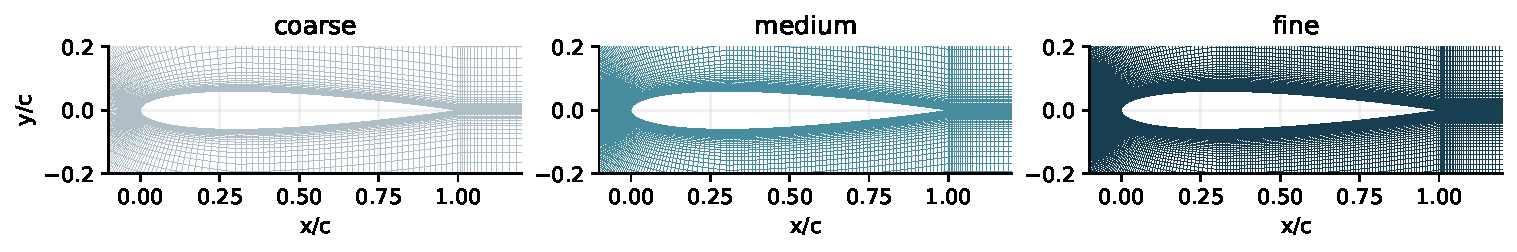
\includegraphics[width=\linewidth]{mesh.pdf}
Actual retained mesh edges from the three p01 cases. The nominal surface comes from the pinned Foundation10 geometry asset. Template and geometry provenance are retained with GPL licensing. Thin-cell/aspect-ratio warnings are not erased; checkMesh logs accompany every case.
\clearpage\section{Wall treatment and numerical gates}
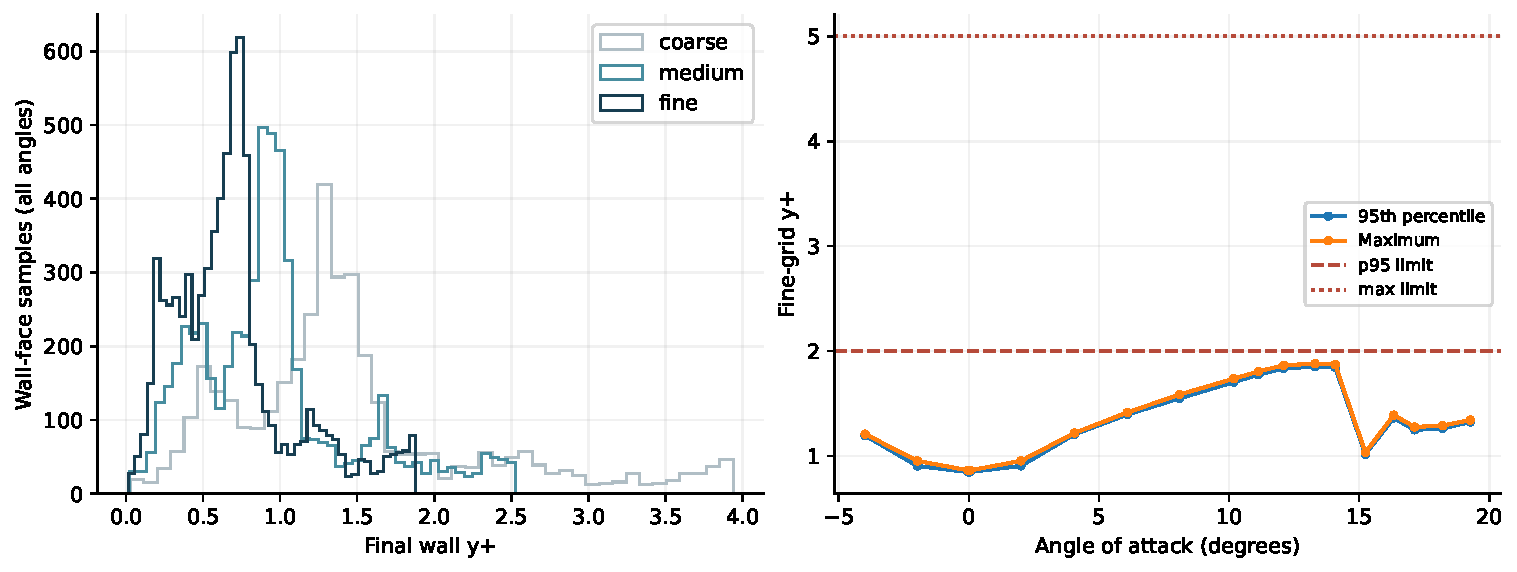
\includegraphics[width=\linewidth]{wall-diagnostics.pdf}
The fine-grid95th-percentile y+ limit is2 and its maximum limit is5. A passing y+ check alone does not establish transition equivalence, turbulence-model adequacy or physical validation. The imposed intermittency band is not a geometrically resolved grit strip.
\subsection{Acceptance policy}
Each case must finish2000 SIMPLE iterations with finite fields and verified trip constraints. Initial residuals at the final iteration must be at most1e-4 and final linear residuals at most1e-6 for the declared fields. Boundary-flux imbalance must be at most0.001; the separate solver-continuity limits remain in preregistration.
Means over iterations1000--1500 and1500--2000 must differ by at most0.01 CL and0.001 CD. Last500-iteration ranges must be at most0.02 CL and0.002 CD. Medium-to-fine differences must be at most0.02 CL and0.002 CD. Iteration means are not physical-time averages.
\clearpage\section{Convergence, conservation and grid sensitivity}
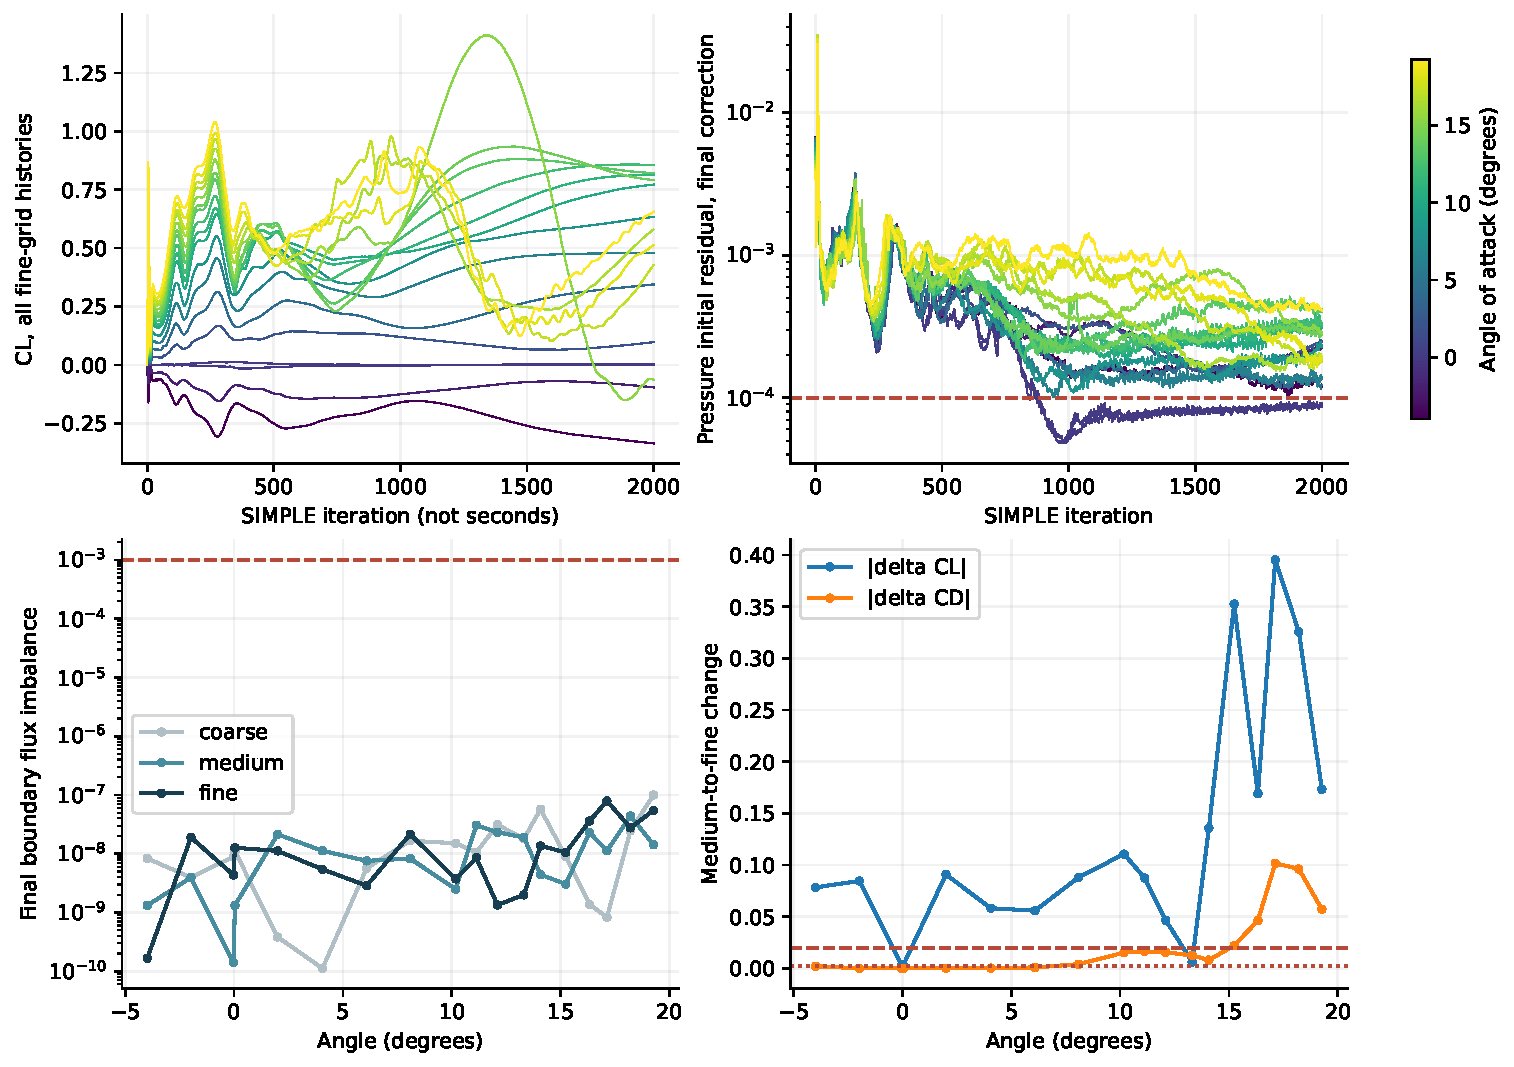
\includegraphics[width=\linewidth]{numerical-evidence.pdf}
Every fine-grid force and pressure-residual history is shown. Boundary flux is independently summed over retained patch fluxes and normalized by total absolute boundary flux; it is not a residual relabeled as conservation. Numerical warnings and failed gates are retained even if the coefficient comparison happens to agree.
\clearpage\section{Frozen prediction versus experiment}
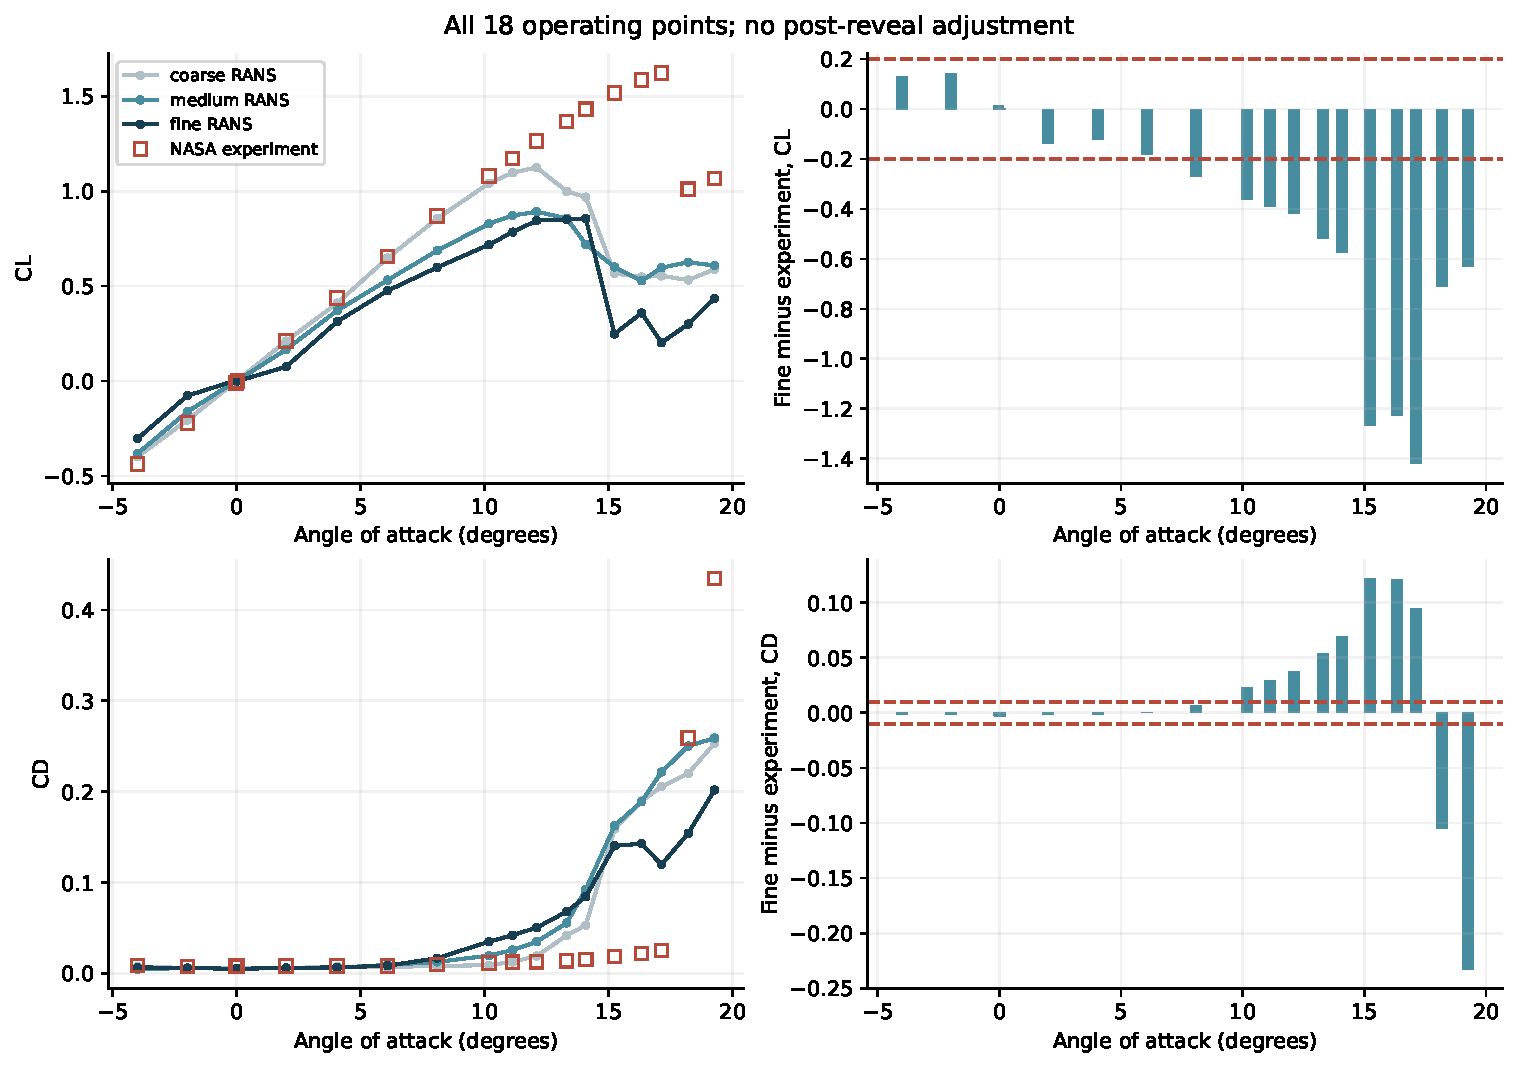
\includegraphics[width=\linewidth]{comparison.pdf}
All points are shown on their registered angles. Dashed error bounds are the preregistered maximum-absolute-error limits. Experimental uncertainty bars are absent because pointwise uncertainty is not supplied. The fine grid supplies the frozen prediction; no grid extrapolation is substituted after reveal.
\clearpage\section{Complete coefficient errors}
\begin{longtable}{rrrrrrr}\toprule $\alpha$ & $C_L$ pred. & $C_L$ exp. & Error & $C_D$ pred. & $C_D$ exp. & Error\\\midrule
-3.99000 & -0.30394 & -0.43630 & 0.13236 & 0.00680 & 0.00871 & -0.00191\\
-1.98000 & -0.07748 & -0.22130 & 0.14382 & 0.00609 & 0.00792 & -0.00183\\
-0.03000 & 0.00229 & -0.01150 & 0.01379 & 0.00521 & 0.00803 & -0.00282\\
0.04000 & -0.00048 & -0.00130 & 0.00082 & 0.00521 & 0.00811 & -0.00290\\
2.00000 & 0.07477 & 0.21130 & -0.13653 & 0.00617 & 0.00814 & -0.00197\\
4.06000 & 0.31296 & 0.43650 & -0.12354 & 0.00680 & 0.00814 & -0.00134\\
6.09000 & 0.47563 & 0.65580 & -0.18017 & 0.00857 & 0.00851 & 0.00006\\
8.09000 & 0.59855 & 0.86890 & -0.27035 & 0.01690 & 0.00985 & 0.00705\\
10.18000 & 0.71838 & 1.08090 & -0.36252 & 0.03499 & 0.01165 & 0.02334\\
11.13000 & 0.78427 & 1.17310 & -0.38883 & 0.04221 & 0.01247 & 0.02974\\
12.10000 & 0.84511 & 1.26440 & -0.41929 & 0.05051 & 0.01299 & 0.03752\\
13.31000 & 0.85120 & 1.36760 & -0.51640 & 0.06813 & 0.01408 & 0.05405\\
14.08000 & 0.85596 & 1.43160 & -0.57564 & 0.08461 & 0.01533 & 0.06928\\
15.24000 & 0.24802 & 1.51690 & -1.26888 & 0.14048 & 0.01870 & 0.12178\\
16.33000 & 0.35868 & 1.58550 & -1.22682 & 0.14284 & 0.02186 & 0.12098\\
17.13000 & 0.20144 & 1.62190 & -1.42046 & 0.11987 & 0.02513 & 0.09474\\
18.21000 & 0.29992 & 1.01040 & -0.71048 & 0.15410 & 0.25899 & -0.10489\\
19.27000 & 0.43528 & 1.06640 & -0.63112 & 0.20179 & 0.43446 & -0.23267\\
\bottomrule\end{longtable}
\subsection{Experimental and numerical outcomes are separate}
Numerical status: FAIL. Experimental comparison: FAIL. Overall status: FAIL. A failed numerical gate prevents an overall PASS regardless of coefficient agreement. This report does not infer a unique physical cause of error from coefficient mismatch alone.
\clearpage\section{Limitations and reproduction}
The study assumes a nominal two-dimensional geometry, low-Mach incompressibility, an assumed inlet turbulence state and a prescribed-transition surrogate. The source does not establish exact as-built coordinates, grit height, series temperature or pointwise coefficient uncertainty. A steady RANS fixed point cannot establish physical steadiness near stall. No transient averaging, spanwise instability resolution or physical grit drag is claimed.
During pre-registration development, rejected O-grid and C-grid attempts exposed mesh-quality and runtime issues. A case-insensitive Phi/phi filename collision was repaired by not exporting the uppercase potential field. The unmodified transition model uses limiting expressions with zero-vorticity denominators: floating-point trapping was disabled, but stored fields and coefficients were required to be finite. These decisions are recorded before production, not hidden post-reveal repairs.
\subsection{Reproduce a case}
\begin{verbatim}python code/execute_case.py NEW_OUTPUT --level fine
  --angle -3.99 --duration 2000 --timeout 7200
\end{verbatim}
Use the pinned public OpenFOAM10 image recorded in preregistration. Every case archive includes generated geometry, mesh, initial/final fields, constraints, decks, logs, coefficient history, extraction results and its own file-hash manifest. Archive hashes are committed with the prediction. Running the code requires Docker and local Python; no model token or private VM access is required.
\subsection{References}
\begin{enumerate}
\item C. L. Ladson. NASA TM-4074 (1988). \url{https://ntrs.nasa.gov/citations/19880019495}.
\item OpenFOAM Foundation, Version10 source and user guide. \url{https://doc.cfd.direct/openfoam/user-guide-v10/}.
\item R. B. Langtry and F. R. Menter (2009), Correlation-based transition modeling for unstructured parallelized CFD codes, AIAA Journal47(12),2894--2906. Model implementation: Foundation10 kOmegaSSTLM.
\end{enumerate}
\clearpage\section{Commitments and artifact identity}
\paragraph{input.json}
{\small\ttfamily\detokenize{827bb840cce7068cd09c0a292aea4efcd73a8d046c18c7e7eb1751fbefce3c73}}
\paragraph{reference.enc}
{\small\ttfamily\detokenize{bc70021062c16133cef3816ddea98a6e9fe54a60c1908ccdf7d03f60bada0184}}
\paragraph{preregistration.json}
{\small\ttfamily\detokenize{d82c98b1f835a52b88c7f355e738253741cb2aa0ae3216913cdad1993c985c6c}}
\paragraph{blind\_prediction.json}
{\small\ttfamily\detokenize{7b5e04d12e2e0be0aaefdec2eb29c1a9728f6f0ddbb90f2d6a72160742638e31}}
\paragraph{comparison.json}
{\small\ttfamily\detokenize{f165ced785f6a23604e579a5b64b71261d80b78fd3c29b51c04befd45f069b46}}
\paragraph{CRITERIA\_FROZEN\_ANCHORED}
\href{https://github.com/alexthegreat714/alex-blythe-site/commit/0fb460ae948d0a11ce39ed565d619d5eb1d78622}{\texttt{0fb460ae948d0a11ce39ed565d619d5eb1d78622}}
\paragraph{PREDICTION\_FROZEN\_ANCHORED}
\href{https://github.com/alexthegreat714/alex-blythe-site/commit/b98e123b11a37bf0f0e0dfae916bfe2d5b4e1507}{\texttt{b98e123b11a37bf0f0e0dfae916bfe2d5b4e1507}}
\paragraph{COMPARED\_ANCHORED}
\href{https://github.com/alexthegreat714/alex-blythe-site/commit/ada06530369cbdd9393cf9432241c0954d916b93}{\texttt{ada06530369cbdd9393cf9432241c0954d916b93}}
\par
Hashes establish identity, not scientific validity or an immutable timestamp against repository administrators. The original frozen prediction and its failures remain preserved. Any later tuning must be published as a separately versioned follow-up.
\end{document}
